\section{Referências Bibliográficas}

\begin{frame}{Referências Bibliográficas}
\begin{itemize}
 \item A forma mais simples de se referenciardentro de um texto é usando o ambiente {\ttfamily thebibliography}.
\item Entretanto, o Bib\TeX{} é uma ferramenta que oferece muito mais flexibilidade na formatação dos textos.
\end{itemize}
\end{frame}

\begin{frame}{Configurando o documento}
\lstinputlisting{pablo/biblio.tex}
\end{frame}

\subsection{Coletando citações}

\begin{frame}{Use o \href{http://scholar.google.com.br}{Google Acadêmico}}
	
\begin{figure}[htbp!]
	\centering
	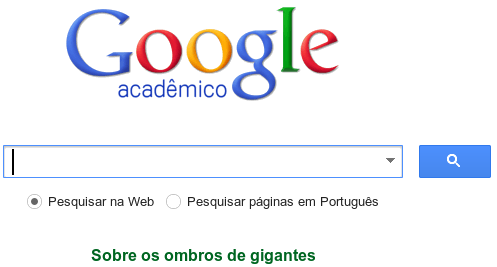
\includegraphics[width=0.6\textwidth]{figuras/google1.png}
	\caption{ }
\end{figure}
\end{frame}

\begin{frame}{Coletando citações}
	
\begin{multicols}{2}
\begin{figure}[htbp!]
	% \centering
	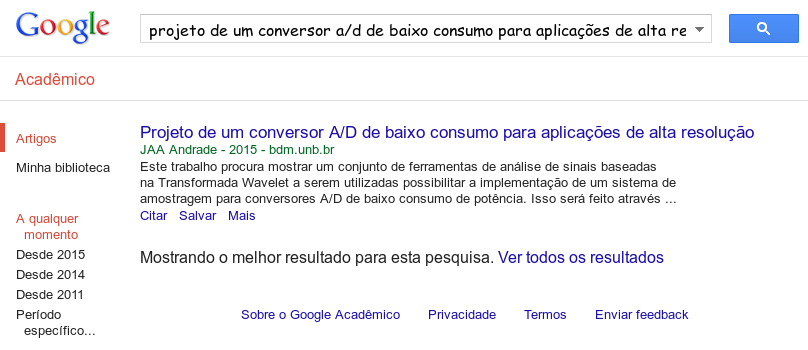
\includegraphics[width=0.6\textwidth]{figuras/google2.png}
	\caption{ }
\end{figure}
	
\begin{figure}[htbp!]
	\centering
	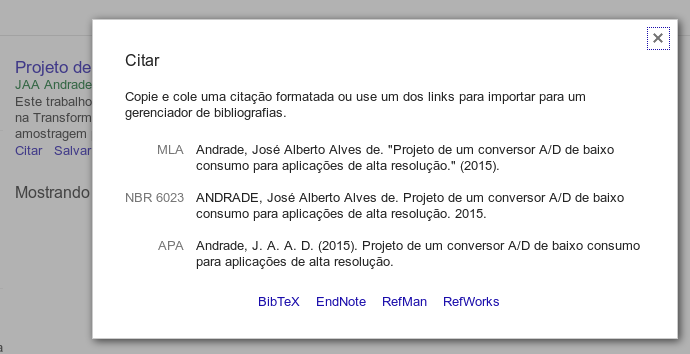
\includegraphics[width=0.4\textwidth]{figuras/google3.png}
	\caption{ }
\end{figure}
\end{multicols}
\end{frame}

\begin{frame}[fragile]{Coletando citações}

\begin{lstlisting}[linewidth=10cm]
@article{andrade2015projeto,
  title={Projeto de um conversor A/D de baixo consumo para aplica{\c{c}}{\~o}es de alta resolu{\c{c}}{\~a}o},
  author={Andrade, Jos{\'e} Alberto Alves de},
  year={2015}
}
\end{lstlisting}
	
\end{frame}